\chapter{Diseño}
\section{GDD (Documento de Diseño de Juego)}

\subsection{Concepto de la aplicación}
ReMind es una plataforma web diseñada para facilitar la gestión y el seguimiento clínico de pacientes que requieren estimulación cognitiva. El sistema permite a los facultativos y terapeutas monitorizar de forma objetiva las actividades realizadas por los pacientes, con el objetivo de preservar y mejorar su salud cognitiva mediante minijuegos desarrollados específicamente para este propósito. El usuario de tipo paciente accede a la plataforma para ejecutar las tareas pautadas por su terapeuta, mientras que el personal médico dispone de herramientas centralizadas para gestionar agendas, prescribir juegos y supervisar la evolución del progreso de forma remota. Esta experiencia digital se ha proyectado para ser intuitiva, accesible y motivadora, reduciendo la frustración y fomentando la adherencia al tratamiento neuropsicológico prescrito.

\subsection{Gameplay}

\subsubsection{Mecánicas generales y arquitectura de interacción}
El sistema fundamenta su interacción en la repetición de tareas cognitivas complementadas con una retroalimentación (\textit{feedback}) directa e inmediata hacia el usuario. Con el propósito de mitigar la fatiga cognitiva y minimizar la barrera de entrada tecnológica propia del público objetivo, el control del juego se restringe a acciones periféricas básicas mediante el ratón o la pantalla táctil: pulsar (\textit{clic / tap}) y arrastrar y soltar (\textit{drag and drop}).

\subsubsection{Mecánicas específicas por módulo}
\begin{enumerate}
    \item \textbf{Módulo 1: Ordenar la secuencia} \\
    \textit{Mecánica:} Ordenación lógica o cronológica de una serie de imágenes. El usuario interactúa con los elementos visuales en pantalla, desplazándolos espacialmente hasta reconstruir la secuencia correcta establecida por el sistema.
    
    \item \textbf{Módulo 2: Relacionar objetos y profesiones} \\
    \textit{Mecánica:} Asociación directa de conceptos afines. El sistema despliega un conjunto de objetos y profesiones, y el usuario debe enlazarlos correctamente (por ejemplo, asociar un estetoscopio con la figura de un médico) mediante la interacción con la pantalla.
    
    \item \textbf{Módulo 3: Pagos exactos} \\
    \textit{Mecánica:} Realización de operaciones aritméticas básicas orientadas a la gestión de dinero real. El sistema propone una cifra económica a pagar, y el usuario debe seleccionar o arrastrar billetes y monedas virtuales hasta alcanzar exactamente dicha cantidad.
    
    \item \textbf{Módulo 4: Vístete} \\
    \textit{Mecánica:} Vestido virtual de un avatar mediante la superposición visual de prendas. Requiere planificación secuencial por parte del usuario, quien debe seguir un orden lógico a la hora de colocar las distintas capas de ropa (por ejemplo, posicionar la ropa interior antes que el pantalón).
    
    \item \textbf{Módulo 5: Completar la oración} \\
    \textit{Mecánica:} Comprensión y completado de textos. Se muestra por pantalla una oración a la que le falta un término. El usuario debe elegir, de entre varias opciones proporcionadas, aquella palabra que dote de sentido sintáctico y semántico a la frase.
    
    \item \textbf{Módulo 6: Intruso} \\
    \textit{Mecánica:} Identificación de elementos discordantes dentro de un grupo homogéneo. Se presenta un conjunto de imágenes o palabras que pertenecen a una misma categoría lógica (frutas, herramientas, etc.), salvo una de ellas. El usuario debe localizar y seleccionar dicho elemento disonante.
\end{enumerate}

\subsubsection{Objetivos y progresión del jugador}
El objetivo principal del usuario es resolver de forma autónoma los ejercicios planteados en su sesión de trabajo. Al tratarse de una herramienta con fines estrictamente terapéuticos, la progresión no se gestiona mediante los sistemas lúdicos tradicionales de puntos, vidas o recompensas, sino mediante un ajuste dinámico de la dificultad. El sistema adapta el nivel del reto modificando variables como:
\begin{itemize}
    \item La cantidad total de elementos mostrados simultáneamente en la interfaz.
    \item La inclusión opcional de límites de tiempo para completar la tarea.
    \item La proximidad semántica o complejidad de los elementos, como ofrecer opciones de palabras más parecidas entre sí para inducir a la discriminación selectiva.
\end{itemize}

\subsubsection{Elementos lúdicos y motivacionales}
Aunque la plataforma tiene un fin terapéutico, se han incorporado ciertos elementos lúdicos para mantener la motivación del paciente durante las sesiones. Cada vez que el usuario completa un ejercicio, recibe una retroalimentación visual positiva mediante iconos y mensajes de ánimo. Al finalizar la sesión, se muestra un resumen con los aciertos obtenidos. Además, si el paciente completa todos los juegos asignados durante una semana, recibe una insignia digital como reconocimiento a su esfuerzo. Estos elementos buscan reforzar la adherencia al tratamiento sin recurrir a mecánicas competitivas o punitivas que podrían generar ansiedad en el usuario.

\subsection{Historia}
Para facilitar la inmersión del paciente en cada actividad y reducir la sensación de estar realizando un examen, se ha asignado una breve historia contextual a cada minijuego. Estas narrativas son sencillas y están inspiradas en situaciones cotidianas, de manera que el usuario pueda sentirse identificado y comprender el propósito de cada ejercicio:

\begin{enumerate}
    \item \textbf{Ordenar la secuencia:} Durante un paseo por el parque, el paciente encuentra una serie de fotografías que representan momentos importantes de su vida. El objetivo es ayudarle a colocarlas en el orden correcto para reconstruir su línea temporal personal.
    \item \textbf{Relacionar objetos y profesiones:} En el mercado del barrio se han mezclado las herramientas de los distintos oficios. El paciente debe ayudar a emparejar cada objeto con la persona que lo usa.
    \item \textbf{Pagos exactos:} Don Manuel va a comprar el pan y la leche. El paciente debe ayudarle a contar el dinero justo para pagar en la tienda.
    \item \textbf{Vístete:} Llueve y hace frío. El paciente debe vestir al personaje colocando las prendas en el orden correcto para que salga a la calle abrigado.
    \item \textbf{Completar la oración:} Los nietos han escrito una carta a sus abuelos pero faltan algunas palabras. El paciente debe elegir la opción correcta para que la carta tenga sentido.
    \item \textbf{El intruso:} Alguien ha dejado un objeto que no pertenece al cajón de la cocina. El paciente debe encontrar cuál es el elemento que no encaja con los demás.
\end{enumerate}

Estas historias se muestran brevemente antes de cada ejercicio y ayudan a contextualizar la tarea sin añadir complejidad ni distraer al usuario de su objetivo terapéutico.

\subsection{Niveles y contenido}

\subsubsection{Estructura de datos y mapas}
El concepto tradicional de ``mapa'' se sustituye por escenas o plantillas funcionales independientes para cada minijuego. El contenido de cada nivel no se encuentra estático en el código (*hardcoded*), sino que se genera de forma dinámica abstrayendo los datos de la interfaz mediante un banco de datos de estímulos reactivos.

\subsubsection{Misiones y desafíos}
Los desafíos se definen como la correcta resolución de los sets de datos cargados en la escena activa. Estos se estructuran según los parámetros detallados en la Tabla~\ref{tab:desafios}.

\begin{table}[htbp]
\centering
\caption{Matriz de especificación de desafíos y escalabilidad por módulo.}
\label{tab:desafios}
\small
\renewcommand{\arraystretch}{1.4}
\begin{tabularx}{\textwidth}{|l|>{\raggedright\arraybackslash}X|>{\raggedright\arraybackslash}X|}
\hline
\textbf{Minijuego} & \textbf{Desafío principal} & \textbf{Factor de escalabilidad (Dificultad)} \\ \hline
Ordenar secuencia & Reconstrucción de la línea temporal. & Número de hitos o imágenes a ordenar. \\ \hline
Relacionar objetos & Asociación correcta de tuplas. & Número de parejas concurrentes en pantalla. \\ \hline
Pagos exactos & Cálculo y manejo de dinero legal. & Cuantía de la cifra y uso de decimales. \\ \hline
Vístete & Planificación motora y lógica. & Número de capas y condiciones climáticas. \\ \hline
Completar oración & Comprensión verbal y semántica. & Longitud de la frase y similitud de distractores. \\ \hline
Intruso & Discriminación y atención selectiva. & Proximidad semántica entre el intruso y el grupo. \\ \hline
\end{tabularx}
\end{table}


\subsubsection{Enemigos}
No existen entidades hostiles ni agentes reactivos artificiales que compitan contra el usuario. El factor de resistencia del sistema está modelado exclusivamente por los propios límites de tiempo parametrizados y las penalizaciones lógicas derivadas de las respuestas erróneas del paciente.

\subsection{Interfaz (UI/UX) y Cuestiones de Usabilidad}

\subsubsection{Arquitectura de pantallas y menús}
El flujo de navegación se ha diseñado bajo el principio de la menor distancia de clics posible, estructurándose en tres niveles jerárquicos esenciales: el portal de acceso público (*Landing Page* y autenticación), el panel principal de control (*Home* diferenciado por rol de usuario) y las vistas específicas de ejecución (módulos de juego y formularios de gestión).

\subsubsection{Elementos del HUD (Heads-Up Display)}
La interfaz en juego se mantiene estática y libre de elementos emergentes intrusivos para evitar la distracción del paciente. Consta de:
\begin{itemize}
    \item Un indicador de progreso textual (ej: ``Ejercicio 3 de 5'').
    \item Un cronómetro digital visible (únicamente en caso de que el nivel configure un límite de tiempo).
    \item Un botón de salida global claramente identificado con un icono estandarizado para interrumpir la sesión y regresar de forma segura al menú principal.
\end{itemize}


\section{Diseño arquitectónico}
El sistema informático desarrollado se fundamenta en un patrón arquitectónico distribuido de tres capas, estructurado bajo un modelo Cliente-Servidor completamente desacoplado. Esta decisión de diseño garantiza la separación de responsabilidades, facilitando la escalabilidad independiente de cada módulo, optimizando el consumo de recursos y mejorando la mantenibilidad global del software.

A continuación, se detallan los tres componentes esenciales que conforman la infraestructura del proyecto:

\subsubsection{Capa de Presentación (Cliente / Frontend)}
La interfaz de usuario y la lógica de presentación se ejecutan por completo en el lado del cliente utilizando el ecosistema Angular. Esta capa se ha diseñado siguiendo el paradigma de Aplicación de una Sola Página (SPA), lo que reduce drásticamente la latencia de navegación al no requerir recargas completas del navegador.

\begin{itemize}
    \item \textbf{TypeScript:} Se emplea como lenguaje de programación principal, aportando un tipado estático que dota al desarrollo de una mayor robustez y minimiza los errores en tiempo de ejecución.
    \item \textbf{HTML5 y CSS3:} Constituyen la estructura semántica y las hojas de estilo base del diseño web.
    \item \textbf{Bootstrap:} Se integra como framework de estilos para agilizar el maquetado y garantizar una interfaz adaptativa, asegurando una correcta visualización en diferentes resoluciones y dispositivos.
\end{itemize}

\subsubsection{Capa de Negocio (Servidor / Backend)}
El núcleo lógico y el procesamiento de datos residen en el servidor, implementado mediante el framework Spring Boot. Esta capa actúa de forma exclusiva como una Interfaz de Programación de Aplicaciones (API RESTful), abstrayéndose por completo de la renderización visual y concentrándose en el cumplimiento de las reglas de negocio y la seguridad.

Su arquitectura interna procesa las solicitudes a través de la siguiente secuencia:
\begin{enumerate}
    \item \textbf{Enrutamiento:} Captura las peticiones entrantes y las redirige al punto de acceso (*endpoint*) correspondiente según el verbo HTTP empleado (GET, POST, PUT, DELETE).
    \item \textbf{Controladores:} Gestionan el flujo de la petición, validan los datos de entrada y coordinan la llamada a los servicios.
    \item \textbf{Servicios:} Bloques modulares donde se ejecutan los algoritmos, reglas de negocio y validaciones críticas del sistema.
    \item \textbf{Data JPA:} Capa de abstracción de datos que interactúa con el sistema de persistencia mediante un mapeo objeto-relacional (ORM), evitando la escritura de consultas SQL manuales y previniendo vulnerabilidades de inyección de código.
\end{enumerate}

\subsubsection{Capa de Persistencia (Base de Datos)}
El almacenamiento de la información de forma estructurada y relacional se delega en \textbf{MySQL}. Esta base de datos interactúa únicamente con la capa de backend a través de conexiones seguras y optimizadas por el ORM, garantizando la integridad referencial, la consistencia de los datos y la ejecución eficiente de transacciones complejas.

\subsection{Flujo de Comunicación y Protocolos}
La interacción entre las capas descritas se realiza de forma estrictamente asíncrona a través de la red, siguiendo un ciclo cerrado de petición y respuesta:

\begin{description}
    \item[Emisión de la solicitud:] Ante cualquier acción del usuario, el cliente Angular genera una petición asíncrona empleando el protocolo seguro \textbf{HTTP/HTTPS} dirigida hacia los \textit{endpoints} específicos expuestos por la API de Spring Boot.
    \item[Procesamiento y transferencia:] El servidor procesa la lógica requerida, interactúa con la base de datos MySQL en caso de ser necesario y emite una respuesta estructurada bajo el estándar de intercambio de datos \textbf{JSON} (\textit{JavaScript Object Notation}).
    \item[Actualización de la interfaz:] El frontend recibe el paquete JSON, procesa la información y actualiza dinámicamente el Modelo de Objetos del Documento (DOM), ofreciendo una experiencia fluida e instantánea al usuario final.
\end{description}

\begin{figure}[H]
    \centering
    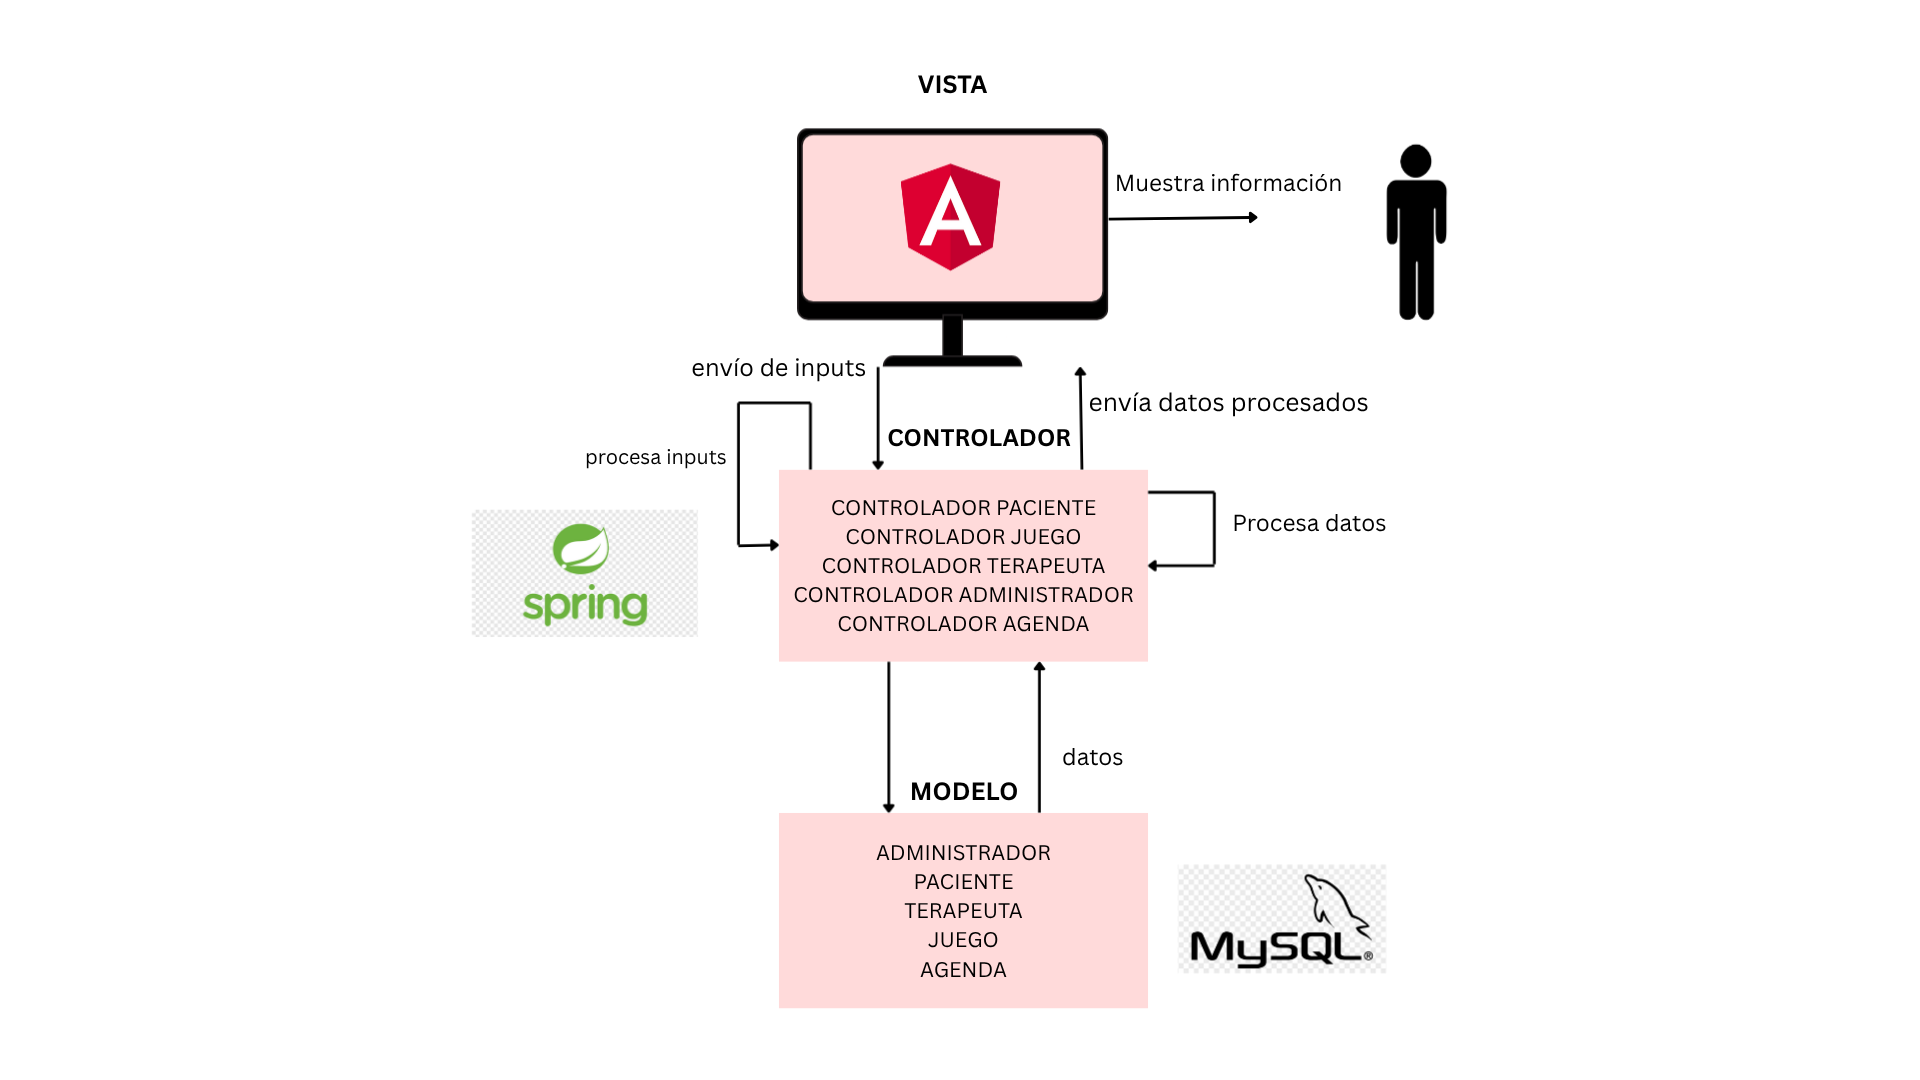
\includegraphics[width=0.9\textwidth]{imagenes/diseno/arquitectura.png}
    \caption{Diagrama arquitectónico de la aplicación.}
    \label{fig:arquitectura}
\end{figure}


\section{Diagrama conceptual del sistema}
En la Figura~\ref{fig:diagrama_conceptual} se detalla el diagrama conceptual de la aplicación, donde se estructuran los diferentes componentes que forman el sistema y cómo se relacionan entre sí. Los elementos de bajo nivel se han omitido deliberadamente para favorecer la legibilidad del modelo.

\begin{figure}[H]
    \centering
    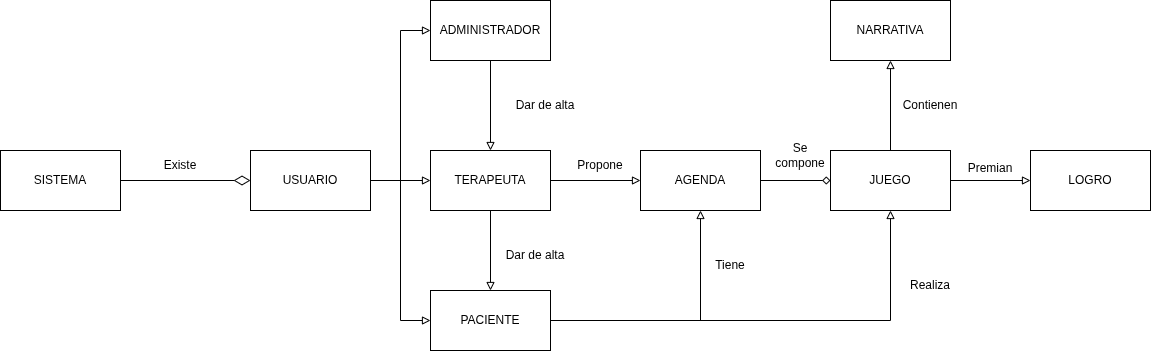
\includegraphics[width=0.9\textwidth]{imagenes/diseno/diagrama_conceptual.png}
    \caption{Diagrama conceptual de la aplicación.}
    \label{fig:diagrama_conceptual}
\end{figure}

El sistema está compuesto por tres roles de usuario perfectamente acotados: pacientes, doctores y administradores. Cada rol tiene asignadas funcionalidades exclusivas dentro de la plataforma. Los doctores realizan la gestión clínica de sus pacientes y administran las agendas de tratamiento. Dichas agendas contienen los minijuegos cognitivos que el paciente debe realizar de forma pautada. Por cada actividad completada con éxito, el paciente recibe una notificación visual en forma de logro para reforzar su motivación. Por último, los administradores poseen la facultad exclusiva de gestionar las cuentas del personal médico, permitiendo dar de alta, editar o eliminar registros de doctores en el sistema.


\section{Diseño de clases y de la base de datos}

\subsection{Diagrama y Entidades de la Base de Datos}
En la Figura~\ref{fig:diagrama_bd} se ilustra el diagrama de la base de datos de ReMind. El sistema se apoya en un modelo relacional para garantizar la flexibilidad, la integridad referencial y la escalabilidad del almacenamiento de datos clínicos.

\begin{figure}[H]
    \centering
    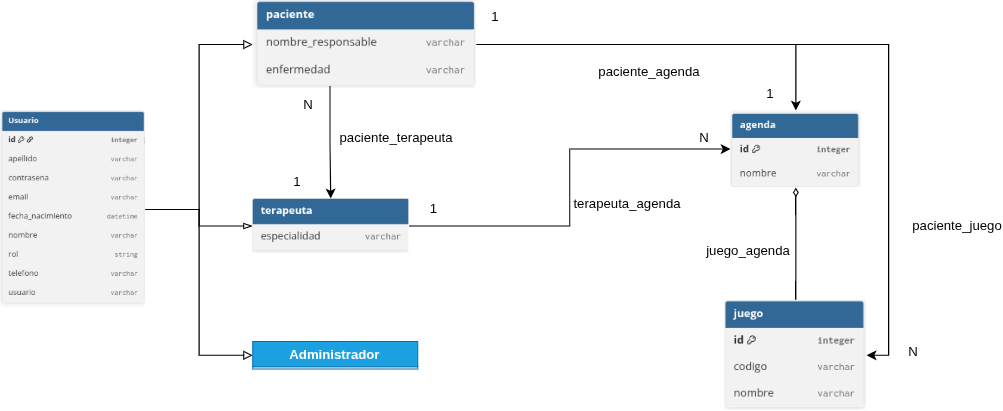
\includegraphics[width=0.9\textwidth]{imagenes/diseno/diagrama_bd.png}
    \caption{Diagrama de clases y base de datos de la aplicación.}
    \label{fig:diagrama_bd}
\end{figure}

A continuación, en la Tabla~\ref{tab:entidades_bd}, se expone la descripción y las relaciones correspondientes a cada una de las entidades fundamentales que componen el esquema de persistencia:

\begin{table}[htbp]
\centering
\small
\caption{Matriz de entidades y relaciones de la base de datos.}
\label{tab:entidades_bd}
\begin{tabularx}{\textwidth}{|l|X|X|}
    \hline
    \textbf{Entidad} & \textbf{Descripción} & \textbf{Relaciones} \\ \hline
    Terapeuta & Almacena la información de registro y credenciales del personal médico. & Relación asociativa con Paciente y Agenda. \\ \hline
    Paciente & Almacena los datos personales e historial clínico del usuario en tratamiento. & Relación con Juego y Agenda. \\ \hline
    Agenda & Define el contenedor temporal de actividades asignado a una planificación. & Vincula de forma directa a Juego, Terapeuta y Paciente. \\ \hline
    Juego & Almacena los parámetros base, rutas y configuraciones de los minijuegos. & Se relaciona con Agenda y Paciente. \\ \hline
    Paciente\_terapeuta & Tabla de unión que vincula de forma unívoca a un paciente con su terapeuta asignado. & Claves foráneas referenciadas a las claves primarias de ambas entidades. \\ \hline
    Agenda\_terapeuta & Tabla asociativa que relaciona al terapeuta con el control de las agendas médicas. & Claves foráneas vinculadas a Terapeuta y Agenda. \\ \hline
    Paciente\_agenda & Relaciona jerárquicamente a un paciente con su correspondiente planificación de tratamiento. & Vinculación mediante el identificador de agenda e identificador de paciente. \\ \hline
    Paciente\_juego & Registra el histórico y estado de los juegos asignados de forma personalizada. & Asociación mediante los identificadores de ambos nodos. \\ \hline
    Juego\_agenda & Estructura el conjunto de minijuegos contenidos dentro de una misma planificación. & Relación indexada por los identificadores correspondientes. \\ \hline
\end{tabularx}
\end{table}


\section{Diseño de la Interfaz y Experiencia de Usuario}
El desarrollo de la capa de presentación se ha articulado bajo el paradigma del Diseño Centrado en el Usuario (DCU). Esta metodología es crítica debido a la naturaleza del público objetivo: pacientes en fases tempranas de enfermedades neurodegenerativas (principalmente Alzheimer). El objetivo de la interfaz consiste en mitigar la carga cognitiva, evitar la desorientación espacial y proporcionar un entorno digital predecible, accesible y emocionalmente seguro.

\subsection{Metodología de Diseño y Evolución}
El flujo de trabajo se dividió en una fase de conceptualización visual (\textit{moodboard}) y una fase de prototipado de media fidelidad (\textit{mockups}). Para el diseño conceptual e iteración rápida de componentes se empleó la herramienta Canva, permitiendo validar contrastes cromáticos iniciales de forma inmediata.

Durante el ciclo de desarrollo, el sistema visual evolucionó para adaptarse a las necesidades del proyecto. El primer ajuste estructural se derivó de la actualización del logotipo de la plataforma, el cual adoptó una tonalidad más oscura. Esto motivó la redefinición de la gama cromática definitiva hacia tonos azules, verdes y naranjas de baja saturación. En las etapas finales del proyecto, la distribución general de la interfaz fue rediseñada para potenciar el carácter profesional de la herramienta, optimizando la visualización de datos de cara a los requisitos de los facultativos y terapeutas (*Product Owners*).

\subsection{Arquitectura de Componentes de la Interfaz y Reutilización}
Siguiendo las directrices de la arquitectura modular, la interfaz se estructura mediante componentes reutilizables en Angular. Vistas complejas, como los paneles de ejercicios didácticos, se subdividen en bloques moleculares comunes (tarjetas de selección, botones de control y barras de estado). Esta estrategia optimiza la base de código del frontend, reduce la redundancia lógica y garantiza una consistencia cognitiva, asegurando que un elemento mantenga estrictamente el mismo comportamiento en cualquier sección de la aplicación para facilitar el aprendizaje del usuario.

Los componentes globales de control, tales como el menú lateral desplegable (*sidebar*) y la barra de navegación superior (*navbar*), se comparten transversalmente en todas las vistas. Del mismo modo, el encabezado indicador de la pantalla se reutiliza de forma constante para favorecer la orientación del usuario dentro de la plataforma. Para la sección de perfiles y formularios, se mantiene una distribución geométrica idéntica: un bloque superior reservado para la identificación e imagen de usuario, y un bloque inferior delimitado para los detalles analíticos o campos de datos asociados.

\subsection{Especificación del Sistema Visual (Moodboard)}
\subsubsection{Tipografía y Legibilidad}
Se ha seleccionado la familia tipográfica \textbf{Roboto} (distribuida a través de Google Fonts) como la fuente base del sistema. La elección se fundamenta en criterios normativos de accesibilidad:
\begin{itemize}
    \item \textbf{Geometría Sans-Serif:} Elimina remates y ornamentos tipográficos innecesarios, reduciendo el ruido visual para usuarios que presentan agudeza visual disminuida.
    \item \textbf{Proporción de la Altura de la X:} Presenta una altura de caja baja elevada, lo que preserva la legibilidad del texto en tamaños reducidos o pantallas de escala variable.
    \item \textbf{Polimorfismo de Grosores:} Permite estructurar una jerarquía de información estricta utilizando una única familia tipográfica, lo que minimiza el esfuerzo de procesamiento visual.
\end{itemize}
\subsubsection{Ingeniería del Color y Accesibilidad Cromática}
La paleta cromática se ha diseñado específicamente para minimizar la fatiga visual y mitigar estados de ansiedad o frustración en el entorno clínico, evitando deliberadamente el uso de colores puros o saturaciones extremas. A continuación, en la Tabla~\ref{tab:sistema_visual}, se detalla la especificación cromática implementada:
\begin{table}[H]
\centering
\small
\renewcommand{\arraystretch}{1.3}
\begin{tabularx}{\textwidth}{|X|X|X|X|}
\hline
\textbf{Elemento de Interfaz} & \textbf{Código HEX} & \textbf{Rol Funcional} & \textbf{Justificación Técnica y Psicológica} \\ \hline
Fondo Principal & \texttt{\#EAF6FF} & Lienzo base & Azul de baja saturación y alta luminosidad. Reduce el contraste estridente del fondo blanco puro y transmite serenidad. \\ \hline
Color Primario & \texttt{\#5A9BD4} & Botones de acción & Azul calmado de intensidad media. Guía el flujo de navegación de forma intuitiva sin generar estrés visual. \\ \hline
Color de Énfasis & \texttt{\#FFF2CC} & Destacados / Avisos & Amarillo suave. Atrae la atención hacia elementos clave sin sobrecargar la percepción del usuario. \\ \hline
Colores Neutros & Escala de Grises & Tipografía/Contenedores & Sustituye al negro puro (\texttt{\#000000}) para suavizar el contraste texto-fondo, previniendo el cansancio ocular. \\ \hline
Color Secundario & \texttt{\#A3D9A5} & Validación y éxito & Verde suave de baja saturación. Indica la resolución correcta de tareas mediante refuerzo positivo. \\ \hline
Color de Alerta & \texttt{\#F4B183} & Notificaciones & Naranja pastel. Captura la atención del usuario de forma amable, evitando el estrés del color rojo estándar. \\ \hline
\end{tabularx}
\caption{Especificación del Sistema Visual e Ingeniería del Color.}
\label{tab:sistema_visual}
\end{table}
\vspace{-\parskip}
\subsubsection{Iconografía}
Para el sistema de iconos se ha integrado la librería \textit{PrimeNG Icons}, respondiendo a los siguientes criterios de ingeniería:
\begin{itemize}
    \item \textbf{Acoplamiento Tecnológico:} Al utilizar el framework de componentes PrimeNG en el desarrollo del frontend, la librería nativa asegura un rendimiento óptimo en el DOM y elimina dependencias externas redundantes.
    \item \textbf{Homogeneidad Estilística:} Dispone de un catálogo uniforme que comparte el mismo grosor de línea y geometría, consolidando la cohesión visual de la plataforma.
\end{itemize}

\subsection{Interacciones Especiales y Pantallas Emergentes}
El flujo de usuario contempla el uso de ventanas modales emergentes en dos escenarios operativos críticos:
\begin{enumerate}
    \item \textbf{Confirmación de Acciones:} Aparecen de forma obligatoria antes de consolidar operaciones de persistencia en la API (como crear, modificar o eliminar usuarios, agendas o citas), actuando como un mecanismo de seguridad ante acciones irreversibles.
    \item \textbf{Valoración de Citas:} Se activa de forma automática cuando el usuario inicia sesión tras concluir el horario de una cita previa, solicitando una calificación inmediata del servicio para recoger datos de control de calidad.
\end{enumerate}

\subsection{Requerimientos de Accesibilidad y Cumplimiento Normativo}
El diseño de la interfaz se rige estrictamente por las pautas \textit{WCAG 2.1} del W3C y las especificaciones de accesibilidad cognitiva \textit{W3C COGA}, aplicando las siguientes restricciones:

\begin{itemize}
    \item \textbf{Ratio de Contraste Lumínico (WCAG 1.4.3):} Se ha verificado que todos los elementos de texto cumplan con el nivel de contraste mínimo AA (4.5:1), alcanzando el nivel AAA (7:1) en los bloques de lectura principales para compensar déficits de agudeza visual.
    \item \textbf{Escalabilidad del Texto (WCAG 1.4.4):} Las fuentes se definen mediante unidades relativas (\texttt{rem}/\texttt{em}), garantizando un diseño fluido que soporta un zoom de hasta el 200\% sin alterar la maquetación ni generar barras de desplazamiento horizontal.
    \item \textbf{Dimensionamiento de Objetivos Táctiles (WCAG 2.5.5 - AAA):} Con el fin de mitigar las limitaciones en la motricidad fina, los elementos interactivos disponen de un área de pulsación mínima de 44x44 píxeles CSS, aislados mediante márgenes de seguridad para prevenir clics accidentales.
    \item \textbf{Consistencia Espacial (WCAG 3.2.3):} Los componentes de navegación conservan una posición fija, semántica idéntica y un patrón visual unificado en todas las pantallas del sistema para reducir el esfuerzo de la memoria a corto plazo.
    \item \textbf{Flexibilidad Temporal (WCAG 2.2.1):} Se descartan las mecánicas basadas en tiempo límite estricto dentro de las actividades cognitivas. Las alertas críticas permanecen visibles en pantalla hasta que medie una acción explícita de cierre por parte del usuario.
\end{itemize}

\subsection{Galería de Prototipos de Interfaz (Mockups)}
Los prototipos se diseñaron pensando en el perfil del usuario final: personas mayores con posible deterioro cognitivo. Por ello, todas las vistas priorizan la simplicidad visual, con pocos elementos en pantalla, botones grandes etiquetados con texto claro, iconos reconocibles y una navegación predecible. Las pantallas de los terapeutas incluyen tablas y filtros para facilitar la gestión de pacientes, mientras que la vista del paciente se limita a mostrar únicamente los juegos disponibles, eliminando cualquier opción innecesaria que pudiera generar confusión. A continuación se muestran las ilustraciones correspondientes al diseño de las vistas principales de la aplicación ReMind:

\begin{figure}[H]
    \centering
    \begin{minipage}{0.48\textwidth}
        \centering
        
\includegraphics[width=\textwidth]{imagenes/mockup/landing.png}
        \caption{Portal de acceso público (*Landing Page*).}
        \label{fig:mockup_landing}
    \end{minipage}
    \hfill
    \begin{minipage}{0.48\textwidth}
        \centering
        
\includegraphics[width=\textwidth]{imagenes/mockup/login.png}
        \caption{Pantalla de autenticación (*Login*).}
        \label{fig:mockup_login}
    \end{minipage}
\end{figure}

\begin{figure}[H]
    \centering
    \begin{minipage}{0.48\textwidth}
        \centering
        
\includegraphics[width=\textwidth]{imagenes/mockup/menu_doctor.png}
        \caption{Panel principal (*Home*) del rol Médico/Doctor.}
        \label{fig:mockup_home_doc}
    \end{minipage}
    \hfill
    \begin{minipage}{0.48\textwidth}
        \centering
        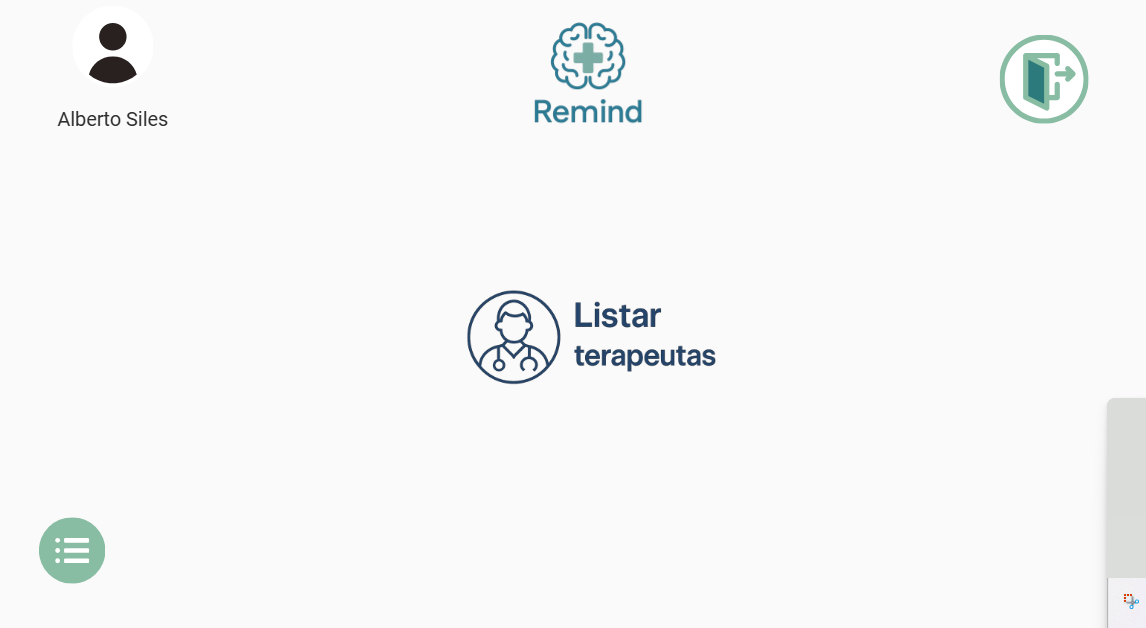
\includegraphics[width=\textwidth]{imagenes/mockup/menu_admiin.png}
        \caption{Panel principal (*Home*) de Administración.}
        \label{fig:mockup_home_admin}
    \end{minipage}
\end{figure}

\begin{figure}[H]
    \centering
    \begin{minipage}{0.48\textwidth}
        \centering
        
\includegraphics[width=\textwidth]{imagenes/mockup/home_paciente.png}
        \caption{Interfaz de inicio del usuario Paciente.}
        \label{fig:mockup_home_paciente}
    \end{minipage}
    \hfill
    \begin{minipage}{0.48\textwidth}
        \centering
        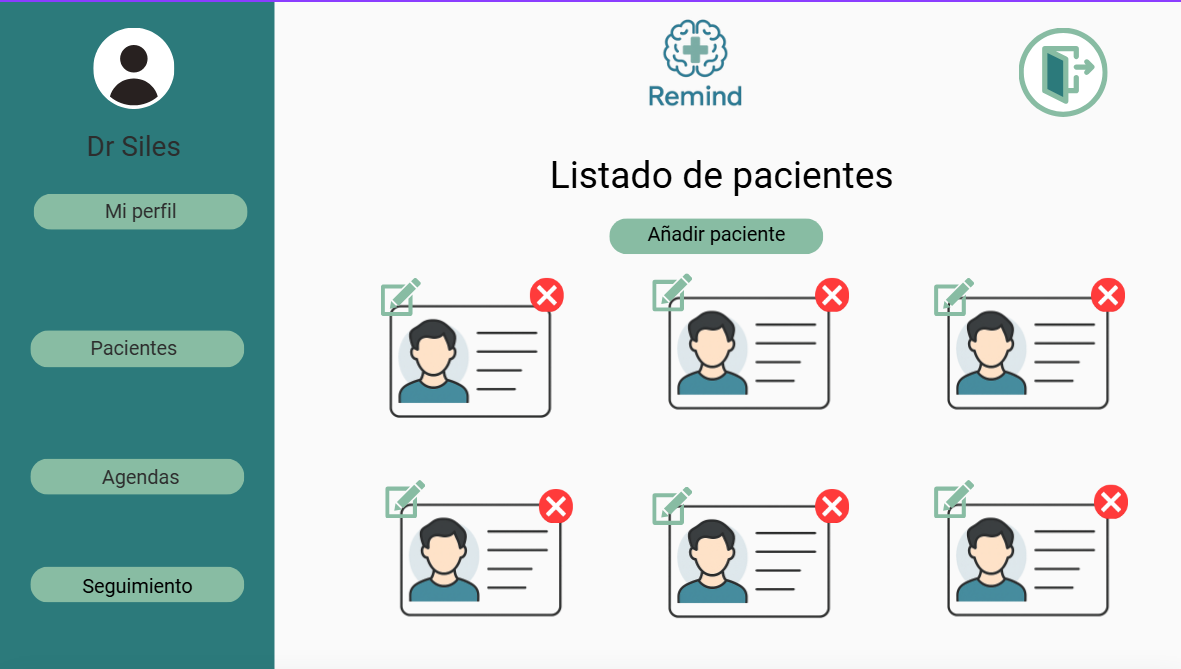
\includegraphics[width=\textwidth]{imagenes/mockup/pacientes.png}
        \caption{Módulo de gestión y selección de pacientes.}
        \label{fig:mockup_gestion_pacientes}
    \end{minipage}
\end{figure}

\begin{figure}[H]
    \centering
    \begin{minipage}{0.48\textwidth}
        \centering
        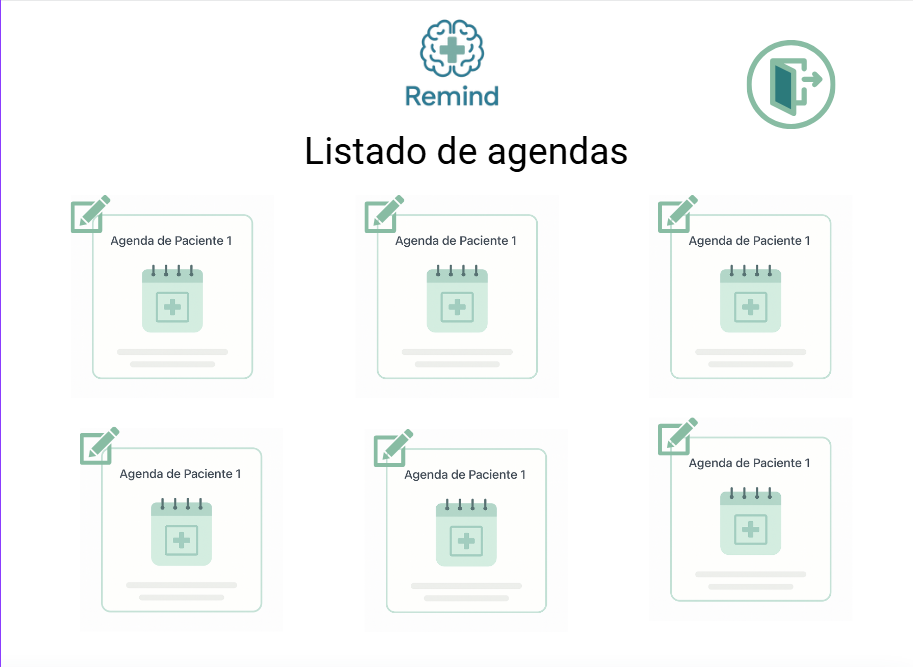
\includegraphics[width=\textwidth]{imagenes/mockup/listar_agendas.png}
        \caption{Listado centralizado de agendas médicas.}
        \label{fig:mockup_lista_agendas}
    \end{minipage}
    \hfill
    \begin{minipage}{0.48\textwidth}
        \centering
        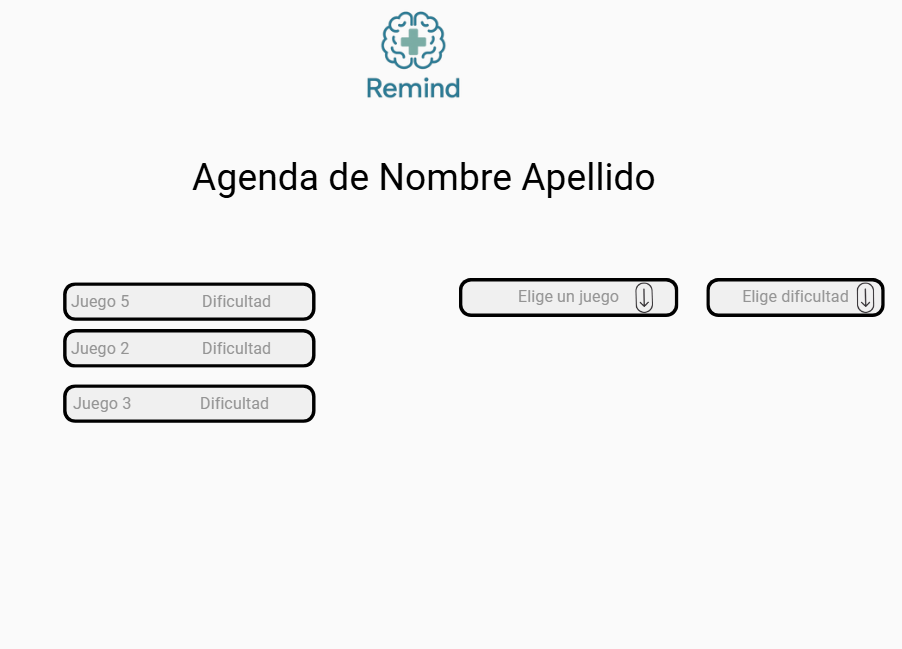
\includegraphics[width=\textwidth]{imagenes/mockup/agenda_paciente.png}
        \caption{Configuración y asignación de actividades.}
        \label{fig:mockup_gestion_agenda}
    \end{minipage}
\end{figure}

\begin{figure}[H]
    \centering
    \begin{minipage}{0.48\textwidth}
        \centering
        
\includegraphics[width=\textwidth]{imagenes/mockup/seguimiento.png}
        \caption{Panel de monitorización y seguimiento clínico.}
        \label{fig:mockup_seguimiento}
    \end{minipage}
    \hfill
    \begin{minipage}{0.48\textwidth}
        \centering
        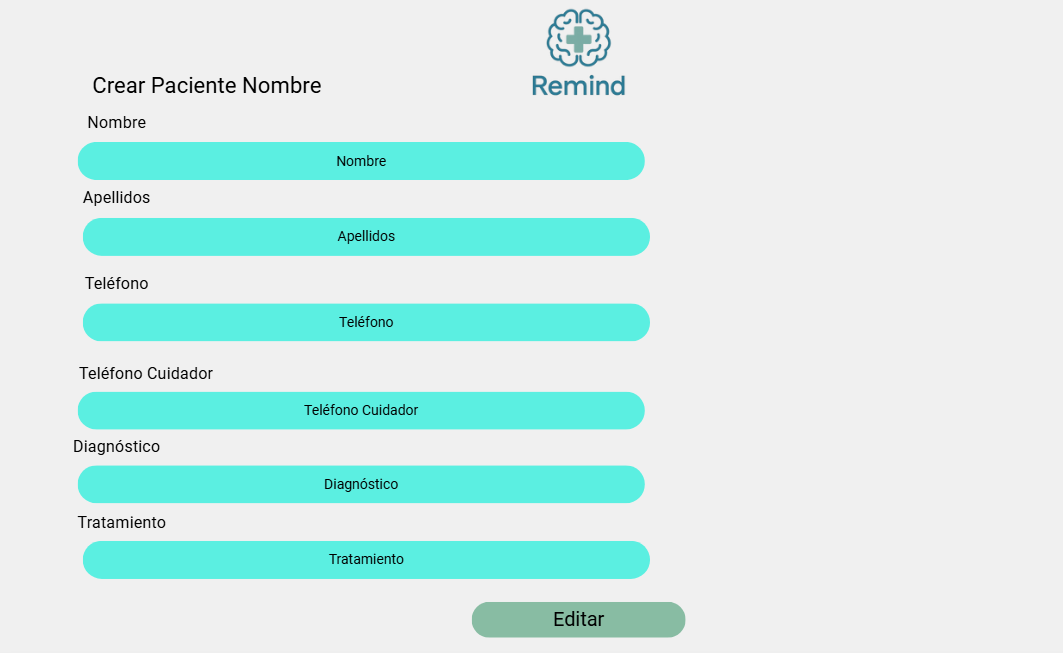
\includegraphics[width=\textwidth]{imagenes/mockup/crear_paciente.png}
        \caption{Diseño del formulario genérico de inserción.}
        \label{fig:mockup_formulario}
    \end{minipage}
\end{figure}